\documentclass[tikz,border=2pt]{standalone}
\renewcommand{\familydefault}{\sfdefault}
\usetikzlibrary{arrows.meta,calc,positioning}
\tikzset{every picture/.style={line width=1pt, >=Stealth},
         hl/.style={fill=black, fill opacity=0.12, text opacity=1}}
\begin{document}
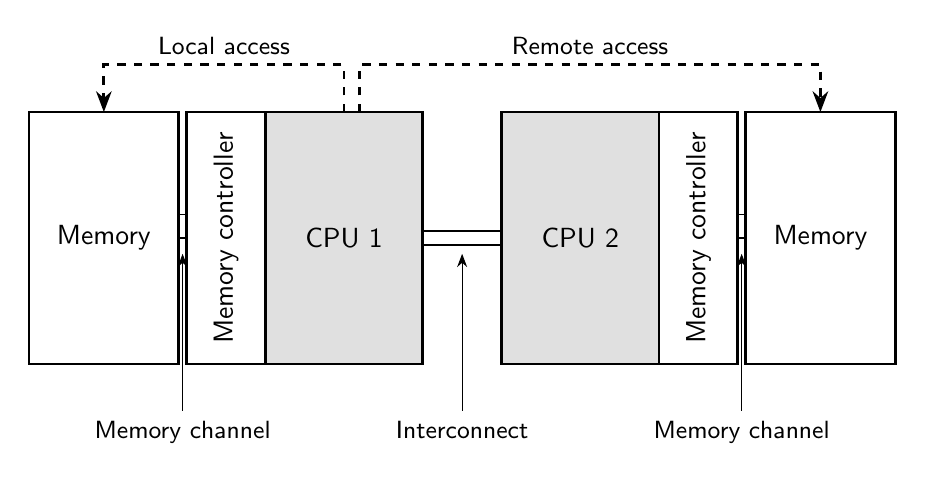
\begin{tikzpicture}[part/.style={draw, minimum height=3.2cm, align=center}]
  % Each CPU reaches its own memory directly, and the other CPU's memory over the interconnect.
  \node[part, minimum width=1.9cm] (mem1) at (0, 0) {Memory};
  \node[part, minimum width=1cm] (mc1) at (1.55, 0) {\rotatebox{90}{Memory controller}};
  \node[part, hl, minimum width=2cm] (cpu1) at (3.05, 0) {CPU 1};
  \node[part, hl, minimum width=2cm] (cpu2) at (6.05, 0) {CPU 2};
  \node[part, minimum width=1cm] (mc2) at (7.55, 0) {\rotatebox{90}{Memory controller}};
  \node[part, minimum width=1.9cm] (mem2) at (9.1, 0) {Memory};
  \foreach \y in {-0.3, 0, 0.3} {
    \draw[thin] (mem1.east |- 0, \y) -- (mc1.west |- 0, \y);
    \draw[thin] (mc2.east |- 0, \y) -- (mem2.west |- 0, \y);
  }
  \draw[double, double distance=4pt] (cpu1) -- (cpu2);

  \draw[->, dashed] (3.05, 1.6) -- (3.05, 2.2) -| node[pos=0.25, above, font=\small] {Local access} (0, 1.6);
  \draw[->, dashed] (3.25, 1.6) -- (3.25, 2.2) -| node[pos=0.25, above, font=\small] {Remote access} (9.1, 1.6);
  \foreach \x/\what in {1/Memory channel, 4.55/Interconnect, 8.1/Memory channel}
    \draw[<-, thin] (\x, -0.2) -- (\x, -2.2) node[below, font=\small] {\what};
\end{tikzpicture}
\end{document}
